\documentclass{article}
\usepackage[utf8]{inputenc}
\usepackage{xeCJK}
\usepackage{indentfirst}
\usepackage{minted}
\usepackage{url}
\usepackage{geometry}
\usepackage{graphicx}
\usepackage{fancyhdr}
% -- page settings
\geometry{a4paper,left=2cm,right=2cm,top=3cm,bottom=2cm}
\renewcommand{\baselinestretch}{1.5}

% -- header & footers
\pagestyle{fancy}
\fancyhf{}
\rhead{\schoolname{}}
\lhead{\classname{}}
\rfoot{\thepage}

% -- defs
\def\schoolname{School of Cyber Engineering, Xidian University}
\def\classname{软件安全与漏洞分析}
\title{\classname{} 大作业}

\author{LIU Jin\\
15180110082 \\
\small{liujin.xdu@pm.me} \and
YANG Chao\\
15180110110 \\
\small{firmianay@gmail.com} \and
LI Yiding\\
15180120028 \\
\small{drimtuer@gmail.com} \and
WANG Xu\\
15130120190 \\
\small{codeklaus@gmail.com}
}

\begin{document}
\maketitle

% STEEINGS
\renewcommand{\contentsname}{目录}
% \renewcommand{\bibname}{参考文献}

% 目录
\newpage
\tableofcontents
\newpage

\begin{center}
    \section{简介}
\end{center}

\setlength{\parindent}{2em}

论文提出了一种不依赖于使用\verb+ return+指令的 ROP 技术。这种攻击方法是在 libc 中找到一些特定的指令序列,来替代 return 指令,完成和\verb+ return+同样的工作。这些指令具备图灵完备性,已经在 (x86)Linux 和 (ARM)Android 中被证实。

由于该攻击方法并不使用\verb+ return+指令,所以那些基于\verb+ return+原理实现的 ROP 防御技术就失效了。

\newpage

\begin{center}
    \section{背景}
\end{center}

正常程序的指令流执行和 ROP 的指令流执行有很大不同,至少存在下面两点:

\begin{itemize}
    \item ROP 执行流会包含了很多\verb+ return+指令,而且这些\verb+ return+指令只间隔了几条其他指令
    \item ROP 利用\verb+ return+指令来 unwind 堆栈,却没有与 ret 指令相对应的 call 指令
\end{itemize}

针对上面两点不同,研究人员提出了很多 ROP 检测和防御技术:
\begin{itemize}
    \item 针对第一点不同,可以检测程序执行中是否有频繁\verb+ return+的指令流,作为报警的依据
    \item 针对第二点不同,可以通过\verb+ call+和\verb+ return+ 指令来查找正常程序中通常都存在的后进先出栈里维护的不变量,判断其是否异常。或者维护一个影子堆栈(shadow stack)作为正常堆栈的备份,每次 return 时对比影子堆栈和正常堆栈是否一致。
    \item 更极端的是,在编译器层面重写二进制文件,消除里面的\verb+ return+指令
\end{itemize}

所以其实这些早期的防御技术都默认了一个前提,即 ROP 中必定存在\verb+ return+ 指令。所以反过来想,如果攻击者能够找到既不使用\verb+ return+指令,又能改变执行流执行任意代码的 ROP 链,那么就成功绕过了这些防御。

\newpage
\begin{center}
    \section{ROP Without Returns}    
\end{center}

于是不依赖于\verb+ return+指令的 ROP 技术诞生了。

我们知道\verb+ return+指令的作用主要有两个:一个是通过间接跳转改变执行流,另一个是更新寄存器状态。

在 x86 和 ARM 中都存在一些指令序列,也能够完成这些工作,它们首先更新全局状态(如栈指针),然后根据更新后的状态加载下一条指令序列的地址,最后跳转过去执行(把它们叫做\verb+ update-load-branch+ 指令序列)。使用这些指令序列完全可以避免 return 指令的使用。

就像下面这样,x 代表任意的通用寄存器:
\begin{minted}[breaklines, frame=lines]{asm}
pop x
jmp *x
\end{minted}

\verb+ r6+通用寄存器里是更新后的状态:
\begin{minted}[breaklines, frame=lines]{asm}
adds r6, #4
ldr r5, [r6, #124]
blx r5
\end{minted}

由于\verb+ update-load-branch+指令序列相比\verb+ return+指令更加稀少,所以需要把它作为 trampoline 重复利用。在构造 ROP 链时,选择以 trampoline 为目标的间接跳转指令结束的指令序列。
当一个 gadget 执行结束后,跳转到 trampoline,trampoline 更新程序全局状态,并将程序控制交给下一个 gadget,由此形成 ROP 链。

% 跳转攻击流程的原理如下图所示:

% \begin{figure}[!h]
%     \centering
%     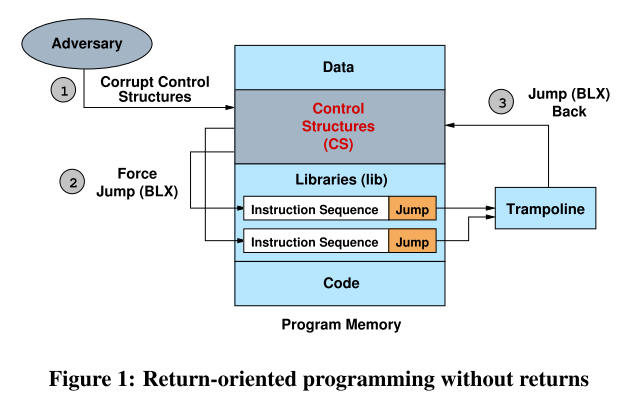
\includegraphics[height=1.5cm]{8.2_rop_without_ret.png}
%     \caption{ROP without returns}
% \end{figure}

在 x86 上,我们使用一个寄存器\verb+ y+保存 trampoline 的地址,那么以间接跳转到\verb+ y+ 结束的指令序列的行为就像是以一个 update-load-branch 指令结束一样。并形成像 ROP 链一样的东西。这种操作在 ARM 上也是类似的。
\newpage

\begin{center}
    \section{x86 上的具体实现}
\end{center}

x86 上的\verb+ return+指令有如下效果:
\begin{itemize}
    \item 检索堆栈顶部的 4 个字节,用它设置指令指针\verb+ eip+
    \item 将堆栈指针\verb+ esp+值增加 4
\end{itemize}

传统的 ROP 就是依靠这个操作将布置到栈上的指令片段地址串起来,依次执行。

现在我们考虑下面的指令序列:
\begin{minted}[breaklines, frame=lines]{asm}
pop %eax; jmp *%eax
\end{minted}

它的行为和\verb+ return+很像,唯一的副作用是覆盖了\verb+ eax+寄存器的内容。现在假设程序的执行不依赖于\verb+ eax+寄存器,那么这一段指令序列就完全可以取代\verb+ return+,这一假设正是本论文的关键。

首先,我们当然可以把\verb+ eax+换成其它任意一个通用寄存器。其次,比起单间接跳转,我们通常使用双重间接跳转:
\begin{minted}[breaklines, frame=lines]{asm}
pop %eax; jmp *(%eax)
\end{minted}

此时\verb+ eax+寄存器存放的是一个被叫做\verb+ sequence catalog+ 表中的地址,该表用于存放各种指令序列的地址,也就是类似于 GOT 表的东西。
第一次跳转,是从上一段指令序列跳到\verb+ catalog+表,第二次跳转,则从\verb+ catalog+ 表跳转到下一段指令序列。这样做使得 ROP 链的构造更加便捷,甚至可以根据某指令序列相对表的偏移来实现跳转。

% 下图是一个函数调用的示例:
% \newpage
% \begin{center}
%     \begin{figure}[!ht]
%         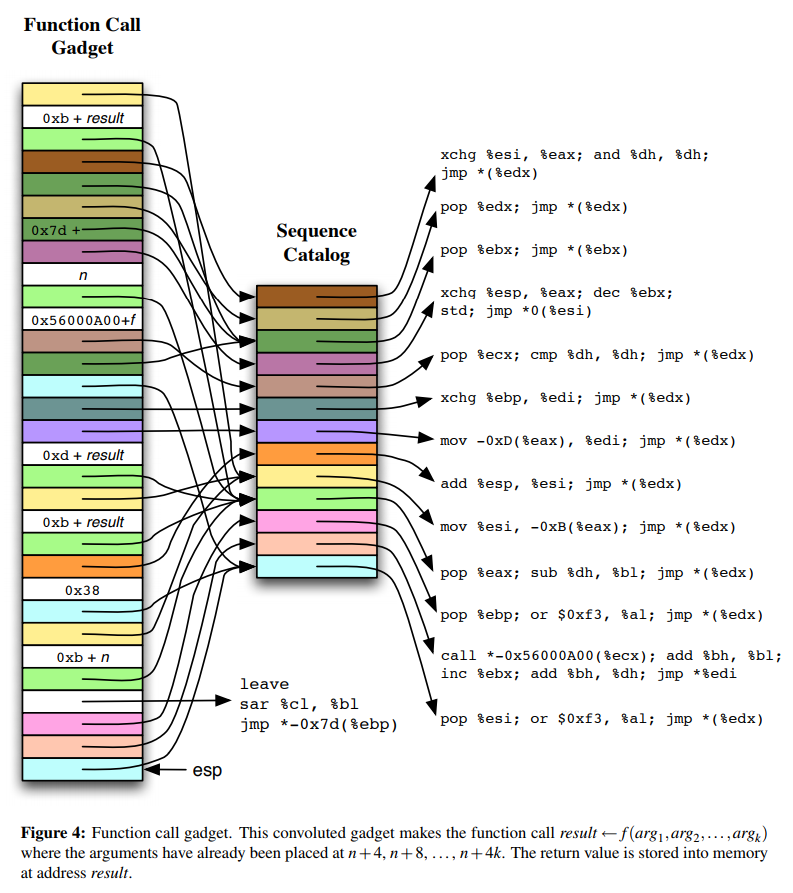
\includegraphics[scale=0.8]{8.2_function.png}
%         \caption{Functions}
%     \end{figure}
% \end{center}


通过 gadget 来实现函数调用一方面可以调用正常的返回导向指令序列,另一方面可以调用合法的函数(需要移动栈指针以及处理返回值)。在函数调用之前,栈指针应该被移动到一个新的位置,以防改写栈上的其他 gadget。
如果函数执行时栈指针位于位置 n,那么 k 个参数应该被保存在\verb| n+4, n+8, ... , n+4k|。然后函数调用 gadget 从而调用函数\verb| A -> fun(arg1, arg2, ..., argn)|。

1. 装载寄存器\verb+ esi+,\verb+ ebp+和\verb+ eax+。
将 catalog 中 call-jump 序列的地址装入 esi 寄存器:
\begin{minted}[breaklines, frame=lines]{asm}
    pop %esi; or $0xf3, %al; jmp *(%edx);
    # call-jump 序列: call *-0x56000A00(%ecx); add %bh, %bl; inc %ebc; add %bj, %dh; jmp *%edi;
\end{minted}
    
将 catalog 中 leave-jump 序列的地址装入\verb+ ebp+寄存器:
\begin{minted}[breaklines, frame=lines]{asm}
    pop %ebp; or $0xf3, %al; jmp *(%edx);
    # leave-jump 序列:leave; sar %cl, %bl; jmp *-0x7d(%ebp);
\end{minted}

将值\verb| 0xb+n|装入\verb+ eax+寄存器:
\begin{minted}[breaklines, frame=lines]{asm}
    pop %eax; sub %dh, %bl; jmp *(%edx);
\end{minted}

2. call-jump 序列的地址位于地址 n,将值\verb+ 0x38+装入寄存器\verb+ esi+,并加上栈指针的值。
此时\verb+ esi+保存了一个地址,在函数调用返回时会将栈指针设置为该地址。
\begin{minted}[breaklines, frame=lines]{asm}
    mov %esi, -0xB(%eax); jmp *(%edx);
    pop %esi; or $0xf3, %al; jmp *(%edx);
    add %esp, %esi; jmp *(%edx);
\end{minted}

3. 将函数返回时栈指针的值赋值给\verb+ ebp+。
先将函数返回的栈指针保存到\verb+ esi+指向的内存中:
\begin{minted}[breaklines, frame=lines]{asm}
    pop %eax; sub %dh, %bl; jmp *(%edx);
    mov %esi, -0xB(%eax); jmp *(%edx);
\end{minted}

将上一步存放的栈指针取出来放入\verb+ edi+寄存器:
\begin{minted}[breaklines, frame=lines]{asm}
    pop %eax; sub %dh, %bl; jmp *(%edx);
    mov -0xD(%eax), %edi; jmp *(%edx);
\end{minted}

通过\verb+ xchg+交换\verb+ edi+和\verb+ ebp+:
\begin{minted}[breaklines, frame=lines]{asm}
    xchg %ebp, %edi; jmp *(%edx);
\end{minted}

此时,\verb+ edi+中保存 leave-jump 序列的地址,\verb+ ebp+保存函数返回后的栈指针地址。

4. 将\verb+ pop %ebx; jmp *(%ebx); +序列的地址装入 \verb+ esi+,保存函数地址的指针(加上偏移量)装入 \verb+ ecx+,将值 n 装入\verb+ eax+。交换\verb+ esp+和\verb+ eax+的值,使得栈指针被设置为 n。
\begin{minted}[breaklines, frame=lines]{asm}
    pop %esi; or $0xf3, %al; jmp *(%edx);
    pop %ecx; cmp %dh, %dh; jmp *(%edx);
    pop %eax; sub %dh, %bl; jmp *(%edx);
    xchg %esp, %eax; dec %ebx; std; jmp *0(%esi);
\end{minted}

5. 由于 n 保存了 call-jump 序列的地址,此时 call-jump 序列被调用,即函数被间接调用。函数返回后,\verb+ eax+ 保存了返回值。由于\verb+ edi+保存了 leave-jump 序列的地址,因此 leave-jump 序列被调用,将\verb+ ebp+赋值给\verb+ esp+,并从栈顶 pop 出新的 ebp:
\begin{minted}[breaklines, frame=lines]{asm}
    pop %ebx; jmp *(%ebx);
    call *-0x56000A00(%ecx); add %bh, %bl; inc %ebc; add %bj, %dh; jmp *%edi;
    leave; sar %cl, %bl; jmp *-0x7d(%ebp);
\end{minted}

此时\verb+ ebp+指向\verb+ pop %ebx; jmp *(%ebx);+,然后 jmp 过去。

6. 将\verb+ eax+里的返回值保存到内存:
\begin{minted}[breaklines, frame=lines]{asm}
    pop %ebx; jmp *(%ebx);
    pop %edx; jmp *(%edx);
    xchg %esi, %eax; and %dh, %dh; jmp *(%edx);
    pop %eax; sub %dh, %bl; jmp *(%edx);
    mov &esi, -0xB(%eax); jmp *(%edx);
\end{minted}

\newpage
\begin{center}
    \section{参考文献}
\end{center}

\begin{thebibliography}{}
\bibitem{1}[1] Return-Oriented Programming without Returns
\bibitem[2]{2} Jump-Oriented Programming: A New Class of Code-Reuse Attack

\end{thebibliography}
\end{document}